\section{Results}
\label{sec:results}

\subsection{3D-DefectBench}
\label{sec:db}

Table~\ref{tab:mcc} gives MCC on the expert-agreement cells.
GeomProbe-LR reached 0.241 (95\% CI [0.041, 0.430]; AUROC 0.695) on fused/incomplete, 0.288 ([0.081, 0.489]; AUROC 0.710) on form/surface, and 0.287 ([0.024, 0.505]; AUROC 0.742) on extra geometry.
The macro MCC over these three defects is 0.272.
The macro over all five geometry defects, the headline summary used by the benchmark, is 0.158, which places the probe 8th of the 15 predictors, between Qwen3.5 397B-A17B (0.162) and Claude Sonnet 4.6 (0.145).
Gemini 3.1 Pro leads that five-defect list at 0.298.
On the three primary defects the best VLMs are higher than the probe: Gemini 2.5 Pro at 0.341 and Gemini 3.1 Pro at 0.335.
Figure~\ref{fig:forest} shows the primary-defect intervals.
The honest summary is that the probe is comparable to mid-tier VLM judges, not that it beats them.
% src: results/main_comparison_expert_agreement.csv; results/macro_mcc.csv; results/RESULTS_milestone1.md

\begin{table}[t]
  \centering
  \caption{Matthews correlation on 3D-DefectBench expert-agreement cells. Macro-3 averages the three primary defects. Macro-5 also averages missing parts and pose/placement. VLM rows use the votes released with the benchmark. Predictors are ordered by macro-5.}
  \label{tab:mcc}
  \small
  \begin{tabular}{lrrrrr}
    \toprule
    Predictor & Fused & Form & Extra & Macro-3 & Macro-5 \\
    \midrule
    Gemini 3.1 Pro & 0.463 & 0.362 & 0.179 & 0.335 & 0.298 \\
    Gemini 2.5 Pro & 0.299 & 0.332 & 0.393 & 0.341 & 0.282 \\
    Gemini 3.1 Flash-Lite & 0.308 & 0.148 & 0.433 & 0.296 & 0.253 \\
    GPT-5.4 & 0.240 & 0.384 & 0.270 & 0.298 & 0.217 \\
    Claude Opus 4.7 & 0.217 & 0.259 & 0.360 & 0.279 & 0.180 \\
    GPT-4o & 0.045 & 0.080 & 0.400 & 0.175 & 0.163 \\
    Qwen3.5 397B-A17B & 0.110 & 0.254 & 0.136 & 0.166 & 0.162 \\
    \textbf{GeomProbe-LR} & \textbf{0.241} & \textbf{0.288} & \textbf{0.287} & \textbf{0.272} & \textbf{0.158} \\
    Generator-only & 0.040 & 0.273 & 0.158 & 0.157 & 0.149 \\
    Claude Sonnet 4.6 & 0.126 & 0.244 & 0.155 & 0.175 & 0.145 \\
    GPT-5 mini & 0.162 & $-0.025$ & 0.412 & 0.183 & 0.142 \\
    Mistral Small 3.1 24B & 0.022 & $-0.154$ & 0.225 & 0.031 & 0.051 \\
    FaceCount-LR & 0.013 & 0.000 & 0.132 & 0.048 & 0.029 \\
    Qwen2.5-VL 7B & $-0.045$ & 0.130 & 0.000 & 0.028 & 0.017 \\
    Claude Haiku 4.5 & 0.000 & $-0.005$ & $-0.047$ & $-0.017$ & 0.014 \\
    \bottomrule
  \end{tabular}
\end{table}
% src: results/main_comparison_expert_agreement.csv; results/macro_mcc.csv

\begin{figure}[t]
  \centering
  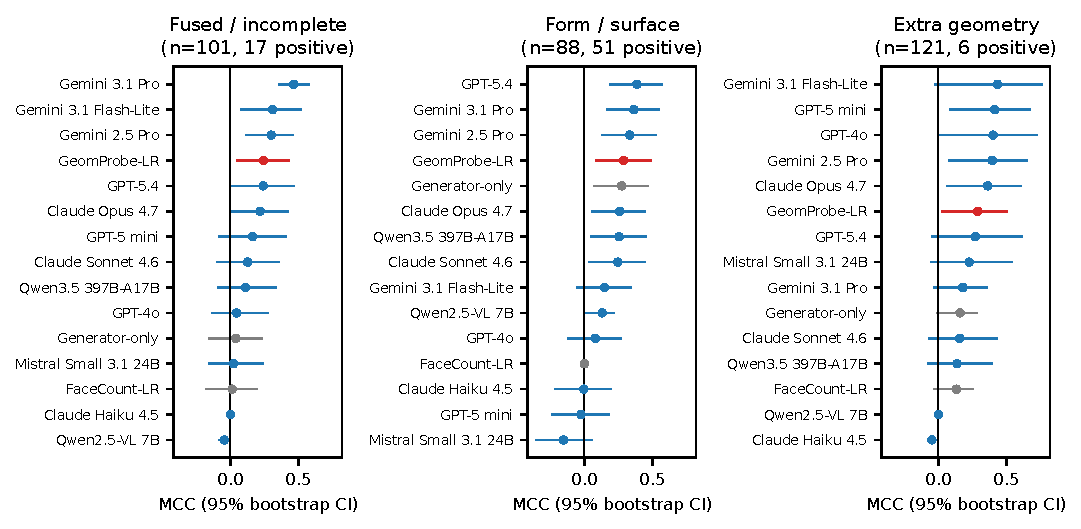
\includegraphics[width=\linewidth]{figures/fig2_forest_mcc.pdf}
  \caption{MCC on the three primary expert-agreement defects, with 95\% asset-bootstrap intervals. GeomProbe-LR is red, the twelve released VLM judges are blue, and the face-count and generator-only controls are grey.}
  \label{fig:forest}
\end{figure}
% src: results/main_comparison_expert_agreement.csv; results/RESULTS_milestone1.md

The paired tests do not support a claim of superiority either way against the strong VLMs.
After false-discovery correction, two of the 36 primary McNemar tests were significant.
The probe was more accurate than Mistral Small 3.1 24B on form/surface (adjusted \(p = 0.044\); \(\Delta\)MCC \(= 0.441\), 95\% CI [0.164, 0.725]).
The probe was less accurate than GPT-4o on extra geometry (adjusted \(p = 0.044\)).
That second contrast is a poor summary of association: GPT-4o predicted one positive against six true positives and its MCC interval is [0.000, 0.722], while the probe predicted 22 positives and the MCC difference has interval \([-0.481, 0.409]\).
One \(\Delta\)MCC interval excludes zero in favour of a strong VLM: Gemini 3.1 Pro on fused/incomplete (\(\Delta\)MCC \(= -0.222\), \([-0.437, -0.014]\)), and the corresponding McNemar test does not (adjusted \(p = 0.960\)).
Intervals that exclude zero in favour of the probe are confined to weaker judges (Claude Haiku 4.5, Qwen2.5-VL 7B, GPT-5 mini and Mistral Small 3.1 24B) and to individual defects.
Against Gemini 2.5 Pro, Gemini 3.1 Pro, GPT-5.4 and Claude Opus 4.7, no primary contrast was significant.
The expert cells are underpowered for those comparisons, particularly extra geometry.
% src: results/paired_tests_probe_vs_vlm.csv; results/main_comparison_expert_agreement.csv; results/RESULTS_milestone1.md

The negative controls behaved as specified.
On missing parts, GeomProbe-LR has MCC 0.024 (\([-0.164, 0.229]\); AUROC 0.570).
Gemini 2.5 Pro reaches 0.430 on the same cells (\(\Delta\)MCC \(= -0.406\), \([-0.741, -0.033]\), adjusted \(p < 0.001\)).
On pose/placement, with two positives, the probe MCC is \(-0.047\).
Face count is a weak control (macro-3 MCC 0.048).
Generator identity is not.
On form/surface the generator-only MCC is 0.273, against 0.288 for the full probe, so that result is largely which of the two generators produced the mesh.
Within-generator probe AUROCs are 0.796 (model A, 32 positives out of 45) and 0.664 (model B, 19 out of 43) for form/surface, 0.786 and 0.597 for fused/incomplete, and 0.785 and 0.705 for extra geometry, the last of these with a single positive in model B.
% src: results/main_comparison_expert_agreement.csv; results/paired_tests_probe_vs_vlm.csv; results/within_generator_auroc.csv; results/RESULTS_milestone1.md

Crowd labels were a poor teacher for form/surface.
Silver out-of-fold AUROC is 0.521 (MCC 0.068) for that defect, against 0.710 on the expert cells, and 0.704 / 0.686 (MCC 0.363 / 0.225) for fused/incomplete and extra geometry.
Classic manifold checks are nearly vacuous on this release: 98.4\% of the 678 GLBs are watertight, none have a non-manifold edge, and 0.4\% have a winding error.
The signals that vary are thin walls, genus, dihedral roughness, self-intersection (47\% of meshes) and hidden surface (49\% of meshes above 1\%), together with small components.
An exploratory scan of single features, selected on the expert cells and therefore optimistic, finds thin-wall fraction at 0.005 with AUROC 0.849 for form/surface and 0.778 for fused/incomplete, and small-component count with AUROC 0.770 for extra geometry.
Thirty-three feature--defect pairs pass a false-discovery threshold of 0.05.
The same ``messiness'' features predict several defect names, so they are not type-specific.
On the secondary target that marks a positive whenever either expert did, over all 129 assets, GeomProbe-LR has MCC 0.424, 0.153 and 0.270 for the three primary defects (AUROC 0.735, 0.640, 0.710).
Generator-only remains comparable on form/surface under that target (MCC 0.154).
% src: results/RESULTS_milestone1.md; results/ablations/expert_trained_on_silver.csv; results/exploratory_feature_auroc.csv; results/secondary_union_target_probes.csv

Figure~\ref{fig:gallery} shows eight meshes chosen by fixed rules, not by visual appeal: the highest probe probability among expert fused/incomplete and extra-geometry positives, the highest fused probability among assets that experts unanimously called free of all three primary defects, the lowest probability among expert form/surface positives, a bottom-decile MATE-3D geometry rating with a large thin-wall fraction, a top-decile rating with a high frozen defect score, and the clean GSO scans with the largest self-intersection and hidden-surface fractions.
The false positive and the high-MOS false alarm are part of the argument, not exceptions tucked out of the figure.
% src: figures/gallery_cases.csv

\begin{figure}[t]
  \centering
  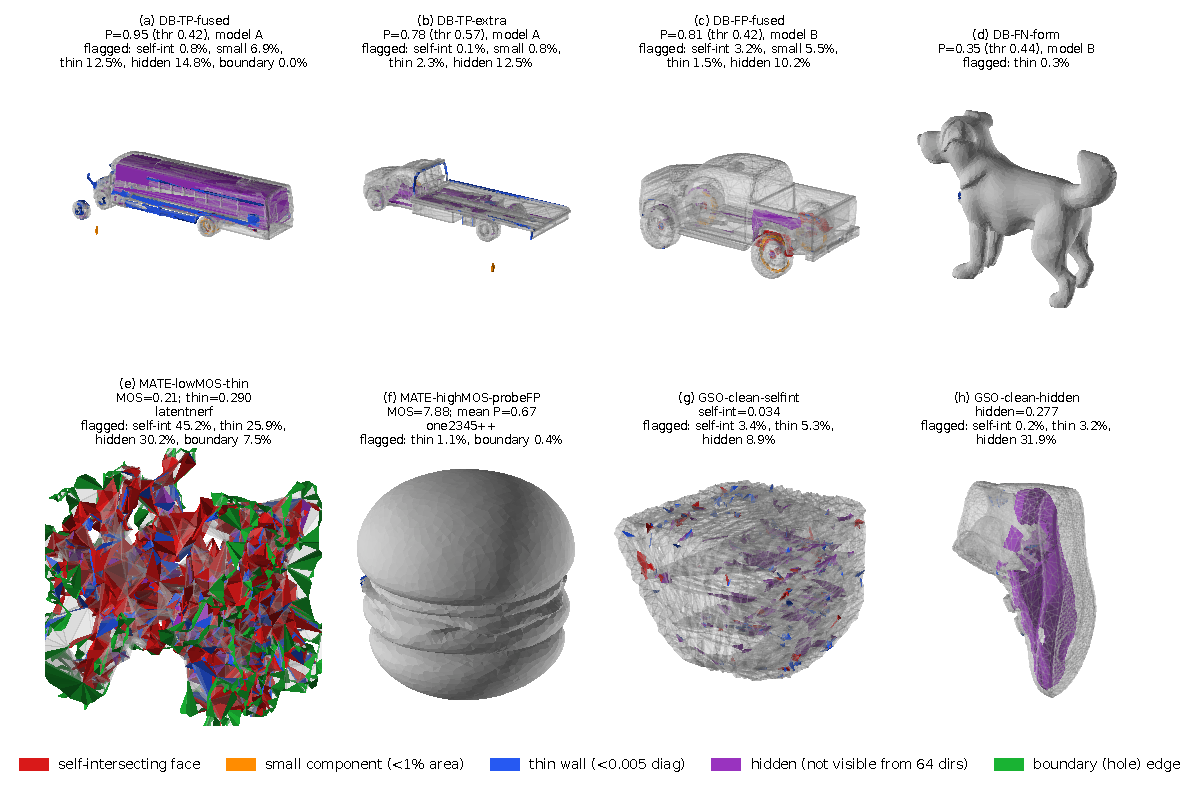
\includegraphics[width=\linewidth]{figures/fig1b_gallery.pdf}
  \caption{Cases selected by fixed rules. (a)~Expert fused/incomplete true positive, probe probability 0.95 against threshold 0.42, model A. (b)~Expert extra-geometry true positive, probability 0.78 against 0.57, model A. (c)~False positive: experts unanimous for no primary defect, fused probability 0.81, model B. (d)~Expert form/surface false negative, probability 0.35 against 0.44, model B. (e)~MATE-3D bottom-decile geometry MOS 0.21 with thin-wall fraction 0.290 (Latent-NeRF). (f)~MATE-3D top-decile MOS 7.88 with mean frozen defect probability 0.67 (One-2-3-45++). (g,h)~Clean GSO scans that already trigger self-intersection (face fraction 0.034) and hidden surface (0.277). Red: self-intersecting face. Orange: small component. Blue: thin wall. Purple: hidden surface. Green: boundary edge. Hidden-heavy meshes are drawn semi-transparent. 3D-DefectBench renders are shown under CC BY-NC 4.0 for non-commercial research.}
  \label{fig:gallery}
\end{figure}
% src: figures/gallery_cases.csv

\subsection{MATE-3D}
\label{sec:mate}

Table~\ref{tab:mate} and Figure~\ref{fig:mate} report the four estimands on the decimated meshes.
Three raw geometric checks replicate under the pre-registered rule.
Within generator, the thin-wall fraction at 0.005 has Spearman \(\rho = -0.195\) (95\% CI \([-0.255, -0.132]\), adjusted \(p = 0.001\)), the genus proxy has \(\rho = -0.110\) (\([-0.165, -0.055]\), adjusted \(p = 0.001\)), and the self-intersection fraction has \(\rho = -0.094\) (\([-0.144, -0.041]\), adjusted \(p = 0.003\)).
The frozen extra-geometry probability (\(\rho = -0.073\), \([-0.132, -0.012]\), adjusted \(p = 0.018\)) and the mean of the three frozen defect probabilities (\(\rho = -0.081\), \([-0.134, -0.027]\), adjusted \(p = 0.010\)) also replicate.
Every one of these within-generator correlations has absolute value at most 0.2.
They are detectable in 1{,}280 meshes and they are small.
% src: results/mate3d/mate3d_dec10k_correlations.csv; results/RESULTS_milestone2.md

\begin{table}[t]
  \centering
  \caption{MATE-3D geometry MOS, decimated meshes (\(n = 1{,}280\)). \(A\) is the pooled Spearman correlation. \(B\) is the within-generator Spearman correlation (primary), with a prompt-cluster interval. \(q\) is the Benjamini--Hochberg value over the nine primary predictors. \(C\) is mean within-prompt Kendall \(\tau\)-b. \(D\) residualises generator and prompt. The predicted sign is negative.}
  \label{tab:mate}
  \resizebox{\linewidth}{!}{%
  \begin{tabular}{lrrrrrl}
    \toprule
    Predictor & \(A\) & \(B\) [95\% CI] & \(q\) & \(C\) & \(D\) & Verdict \\
    \midrule
    Thin fraction (0.005) & $-0.181$ & $-0.195$ [$-0.255$, $-0.132$] & 0.001 & $-0.114$ & $-0.144$ & replicates \\
    Genus proxy & $-0.322$ & $-0.110$ [$-0.165$, $-0.055$] & 0.001 & $-0.263$ & $-0.118$ & replicates \\
    Self-intersection fraction & $-0.291$ & $-0.094$ [$-0.144$, $-0.041$] & 0.003 & $-0.245$ & $-0.057$ & replicates \\
    Dihedral mean & $-0.293$ & $-0.041$ [$-0.103$, $0.020$] & 0.191 & $-0.241$ & $-0.052$ & partial \\
    Hidden-surface fraction & $-0.297$ & $+0.028$ [$-0.033$, $0.088$] & 0.318 & $-0.257$ & $-0.041$ & partial \\
    \(P\)(form/surface) & $+0.150$ & $-0.046$ [$-0.108$, $0.018$] & 0.161 & $+0.120$ & $-0.052$ & fails \\
    \(P\)(fused/incomplete) & $-0.052$ & $-0.035$ [$-0.092$, $0.023$] & 0.234 & $-0.060$ & $-0.042$ & partial \\
    \(P\)(extra geometry) & $-0.218$ & $-0.073$ [$-0.132$, $-0.012$] & 0.018 & $-0.181$ & $-0.094$ & replicates \\
    Mean defect score & $+0.011$ & $-0.081$ [$-0.134$, $-0.027$] & 0.010 & $0.000$ & $-0.114$ & replicates \\
    \bottomrule
  \end{tabular}}
\end{table}
% src: results/mate3d/mate3d_dec10k_correlations.csv; results/RESULTS_milestone2.md

\begin{figure}[t]
  \centering
  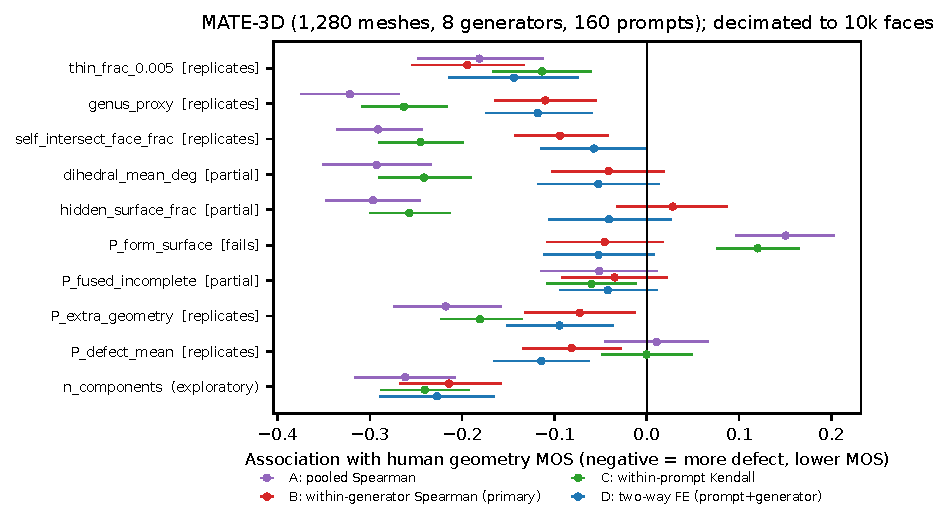
\includegraphics[width=\linewidth]{figures/fig5_mate3d_estimands.pdf}
  \caption{MATE-3D estimands for the nine primary predictors and, as an exploratory addition, component count. \(A\) pools all meshes. \(B\) is within generator and is the pre-registered primary. \(C\) is within prompt. \(D\) removes generator and prompt means. Negative values mean that a larger probe score accompanies a lower human geometry rating.}
  \label{fig:mate}
\end{figure}
% src: results/mate3d/mate3d_dec10k_correlations.csv; results/RESULTS_milestone2.md

Dihedral roughness and hidden surface are the cautionary rows.
Both have pooled correlations near \(-0.29\), and both lose that association once the generator is held fixed (dihedral \(\rho = -0.041\), interval including 0; hidden \(\rho = +0.028\)).
Across the eight generator means the same two features still look strongly related to mean MOS (descriptive Spearman \(-0.833\) and \(-0.762\), \(n = 8\)).
Generators that are rough or internally hidden are rated worse as generators.
Inside a generator, those two measurements do not track the rating.
The frozen form/surface probability fails outright: its pooled correlation is positive (\(+0.150\)), which is the wrong sign for a defect score.
The frozen fused/incomplete probability is only partial (\(\rho = -0.035\), interval including 0).
% src: results/mate3d/mate3d_dec10k_correlations.csv; results/RESULTS_milestone2.md

Figure~\ref{fig:heatmap} shows that the within-generator effects are not shared evenly.
The thin-wall correlation is \(-0.479\) for Latent-NeRF, \(-0.406\) for One-2-3-45++ and \(-0.313\) for SJC, and \(+0.073\) for Magic3D.
Dihedral mean is \(-0.431\) for One-2-3-45++ and \(-0.352\) for Latent-NeRF, and \(+0.257\) for both DreamFusion and TextMesh.
Hidden surface is \(+0.308\) for SJC.
A probe that is averaged over generators will describe a mixture of these regimes.
% src: results/mate3d/mate3d_dec10k_per_generator.csv; results/RESULTS_milestone2.md

\begin{figure}[t]
  \centering
  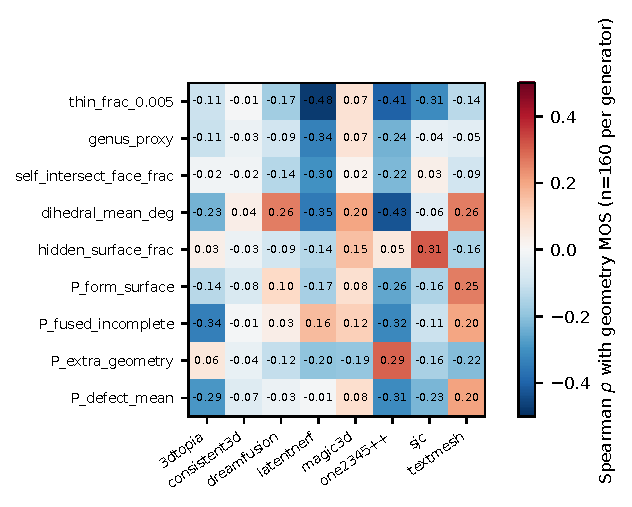
\includegraphics[width=\linewidth]{figures/fig6_mate3d_per_generator.pdf}
  \caption{Per-generator Spearman correlation between each pre-registered predictor and human geometry MOS on MATE-3D. Each column has 160 prompts. The sign is not stable across generators.}
  \label{fig:heatmap}
\end{figure}
% src: results/mate3d/mate3d_dec10k_per_generator.csv

Exploratory component features, which were not in the primary family of nine, have slightly larger within-generator correlations: component count \(\rho = -0.214\), large-component count \(\rho = -0.199\), and largest-component area fraction \(\rho = +0.192\), all with adjusted \(p < 0.001\) under the exploratory correction.
We do not promote them to a confirmed finding on the strength of this one corpus.
The undecimated meshes support the same verdicts for thin walls (\(-0.178\)), genus (\(-0.109\)), self-intersection (\(-0.063\)) and the mean defect score (\(-0.211\)).
Dihedral mean and hidden surface again fail within generator.
The form/surface probability again fails.
The fused/incomplete probability replicates only weakly (\(-0.060\), adjusted \(p = 0.048\)).
Decimation did not create the pattern.
% src: results/mate3d/mate3d_dec10k_correlations.csv; results/mate3d/mate3d_raw_correlations.csv; results/RESULTS_milestone2.md

\subsection{Injected defects on real scans}
\label{sec:gso}

Table~\ref{tab:gso} and Figure~\ref{fig:gsosev} give detection against the 120 clean decimated scans.
Holes and floaters are separated from the clean meshes with AUROC 1.000 at every severity, by boundary-edge fraction and by small-component count respectively.
At a threshold of zero both checks have sensitivity 1.00 and specificity 1.00: the clean decimated scans simply do not contain those signals, and every injected mesh does.
Self-intersection detects interpenetrating parts at AUROC 0.971, 0.978 and 0.986 and crossing sheets at 0.940, 0.965 and 0.977.
Hidden surface detects internal shells at 0.811, 0.869 and 0.912 and interpenetration at 0.835, 0.897 and 0.937.
Noise is visible in the dihedral mean at 0.753, 0.971 and 0.999.
Thin fins at S2 and S3 reach AUROC 0.952 on the 0.005 thin-wall fraction.
The S1 fin, which is thicker than that threshold, is at 0.651; the 0.010 thin-wall fraction reaches AUROC 0.826 on the same S1 fins.
Figure~\ref{fig:gsoex} shows one object, the alphabetically first scan for which all 22 variants probed successfully, at S3.
% src: results/gso/gso_detection.csv; results/RESULTS_milestone2.md; figures/gso_example_object.json

\begin{table}[t]
  \centering
  \caption{GSO injection. AUROC of the pre-registered target check against 120 clean meshes. Sensitivity and specificity are at a strict threshold of zero and are constant across severities for these checks. The S1 fin is thicker than 0.005 by design.}
  \label{tab:gso}
  \small
  \begin{tabular}{llcccc}
    \toprule
    Injected defect & Target check & S1 & S2 & S3 & Sens./spec.\ at 0 \\
    \midrule
    Holes & Boundary-edge fraction & 1.000 & 1.000 & 1.000 & 1.00 / 1.00 \\
    Floaters & Small-component count & 1.000 & 1.000 & 1.000 & 1.00 / 1.00 \\
    Interpenetrating part & Self-intersection & 0.971 & 0.978 & 0.986 & 1.00 / 0.79 \\
    Interpenetrating part & Hidden surface & 0.835 & 0.897 & 0.937 & 1.00 / 0.58 \\
    Crossing sheet & Self-intersection & 0.940 & 0.965 & 0.977 & 1.00 / 0.79 \\
    Hidden shell & Hidden surface & 0.811 & 0.869 & 0.912 & 1.00 / 0.58 \\
    Thin fin & Thin fraction (0.005) & 0.651 & 0.952 & 0.952 & 0.98--1.00 / 0.27 \\
    Noise & Dihedral mean & 0.753 & 0.971 & 0.999 & n/a \\
    \bottomrule
  \end{tabular}
\end{table}
% src: results/gso/gso_detection.csv; results/RESULTS_milestone2.md

\begin{figure}[t]
  \centering
  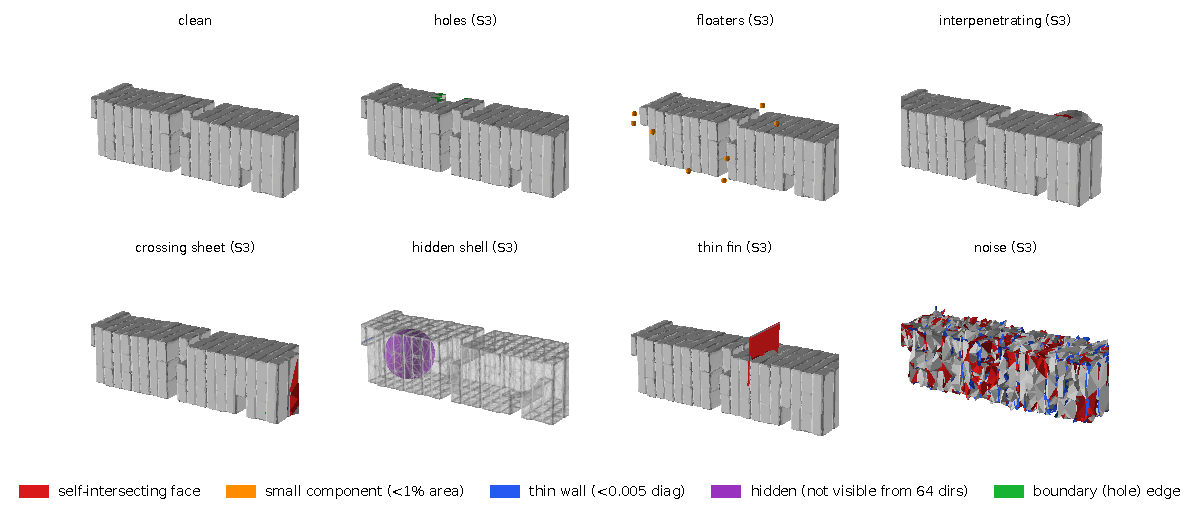
\includegraphics[width=\linewidth]{figures/fig3a_gso_examples.pdf}
  \caption{Clean decimated scan and the seven injected defects at severity S3 for one GSO object (alphabetically first with all 22 variants probed). The operators are applied to the real scan; they are not generator failures.}
  \label{fig:gsoex}
\end{figure}
% src: figures/gso_example_object.json; results/RESULTS_milestone2.md

\begin{figure}[t]
  \centering
  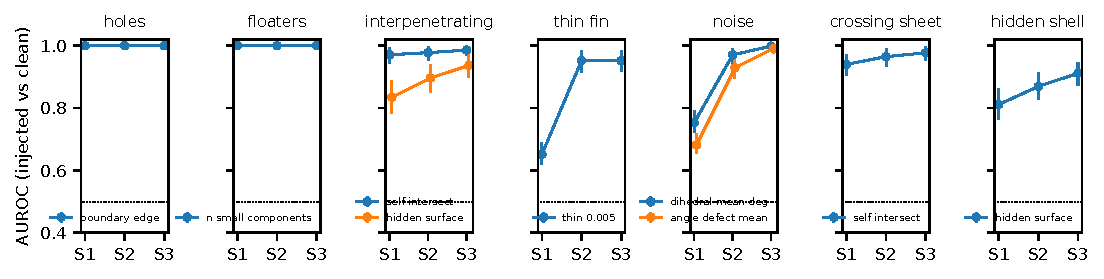
\includegraphics[width=\linewidth]{figures/fig3_gso_severity.pdf}
  \caption{AUROC of each pre-registered target check as injection severity increases from S1 to S3. Holes and floaters are saturated at S1. The thin-fin curve uses the 0.005 threshold, which is below the S1 plate thickness.}
  \label{fig:gsosev}
\end{figure}
% src: results/gso/gso_detection.csv

Specificity at zero is the first place validity and ``clean'' diverge.
Of the clean decimated scans, 21\% already self-intersect, 42\% have hidden-surface fraction above zero, and 73\% have thin-wall fraction above zero, so the strict self-intersection, hidden-surface and thin-wall checks have specificities 0.79, 0.58 and 0.27.
A zero threshold is a property of the decimated scan, not a certificate that a rater would call the mesh clean.

The calibrated thresholds move the operating point to the other extreme.
On the 200 crowd-labelled defect-free 3D-DefectBench assets, the 95th percentile is 0.044 of faces self-intersecting, hidden-surface fraction 0.128, 3.05 small components, thin-wall fraction 0.050, and genus proxy 48.1.
Sensitivity at this \(\tau_c\) is at most 0.10 for the self-intersection targets, at most 0.32 for the hidden-surface targets, and 0 for one and for three floaters (the ten-floater severity does cross 3.05).
Figure~\ref{fig:ecdf} plots the two reference distributions.
Generated assets that the crowd called defect-free sit far to the right of the clean scans.
A gate set on human ``defect-free'' labels will pass meshes that a strict geometric definition rejects, and a strict gate will reject meshes that raters accept.
% src: results/gso/tau_calibrated.json; results/gso/gso_detection.csv; results/RESULTS_milestone2.md

\begin{figure}[t]
  \centering
  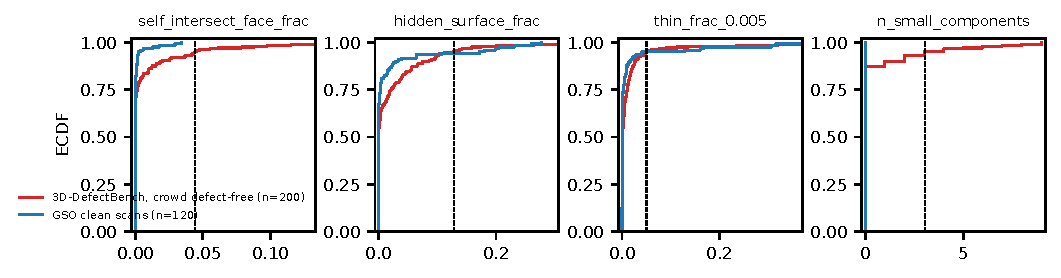
\includegraphics[width=\linewidth]{figures/fig7_ecdf_clean_reference.pdf}
  \caption{Empirical distributions of four checks on crowd-labelled defect-free 3D-DefectBench assets (\(n = 200\)) and on clean decimated GSO scans (\(n = 120\)). Dashed lines are the calibrated thresholds \(\tau_c\), the 95th percentile of the crowd-labelled defect-free set.}
  \label{fig:ecdf}
\end{figure}
% src: results/gso/tau_calibrated.json; results/RESULTS_milestone2.md

The checks are sensitive and, except for holes and floaters, not type-specific.
Figure~\ref{fig:cross} is the S2 cross-talk matrix.
At S3, hidden-surface fraction responds to interpenetration (AUROC 0.94), crossing sheets (0.89), noise (0.86) and thin fins (0.89), not only to hidden shells (0.91).
Self-intersection responds to noise (1.00) and to fins (0.96) as well as to the two operators aimed at it.
Boundary fraction and small-component count stay near chance off their own targets, with one mechanical exception: a crossing sheet also creates a boundary, so boundary fraction detects it at AUROC 1.000.
% src: results/gso/gso_crosstalk_auroc.csv; results/RESULTS_milestone2.md

\begin{figure}[t]
  \centering
  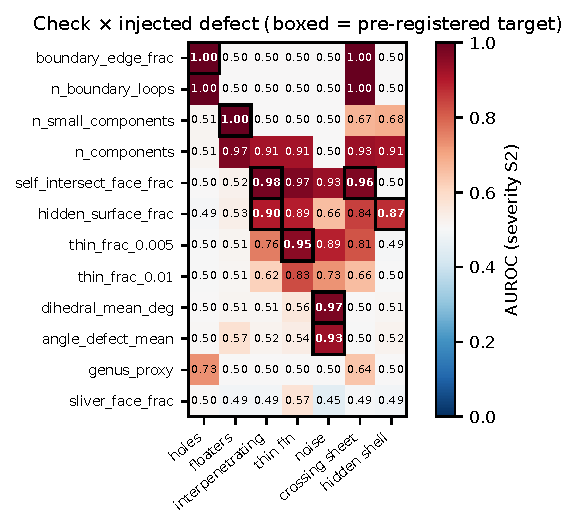
\includegraphics[width=\linewidth]{figures/fig4_gso_crosstalk.pdf}
  \caption{AUROC of each check (rows) against each injected defect at severity S2 (columns). Boxed cells are the pre-registered targets. Off-target cells near 1 show cross-talk; cells near 0.5 show that the check did not move.}
  \label{fig:cross}
\end{figure}
% src: results/gso/gso_crosstalk_auroc.csv

\subsection{Ablations and fusion}
\label{sec:ablate}

Family-only models, trained on the silver holdout and scored on the expert-agreement cells, put most of the expert-set AUROC in the topology family.
Topology alone (six features) reaches AUROC 0.801, 0.770 and 0.786 on fused/incomplete, form/surface and extra geometry (MCC 0.395, 0.572, 0.188), at or above the full 30-feature model (AUROC 0.695, 0.710, 0.742).
Boundary and manifold features alone sit near chance (AUROC 0.564, 0.533, 0.573), which matches the watertightness of this benchmark.
Leave-one-family-out changes AUROC by at most about 0.06.
MCC is less stable than AUROC, because the silver out-of-fold threshold is fragile: dropping self-intersection or triangle quality from the form/surface model pushes that threshold to 1.0 and the expert MCC to 0.
Single-feature rules chosen after seeing the expert set---and therefore optimistic---give genus AUROC 0.763, hidden surface 0.755 and self-intersection 0.698 for fused/incomplete; thin walls 0.849 and dihedral mean 0.691 for form/surface; and small-component count 0.770 for extra geometry.
Choosing the topology-only model because it won on the expert cells would be test-set selection.
We report it as an ablation.
The pre-registered model remains the 30-feature regression.
Figure~\ref{fig:ablate} summarises the family AUROCs.
% src: results/ablations/lofo_family_rules.csv; results/RESULTS_milestone2.md

\begin{figure}[t]
  \centering
  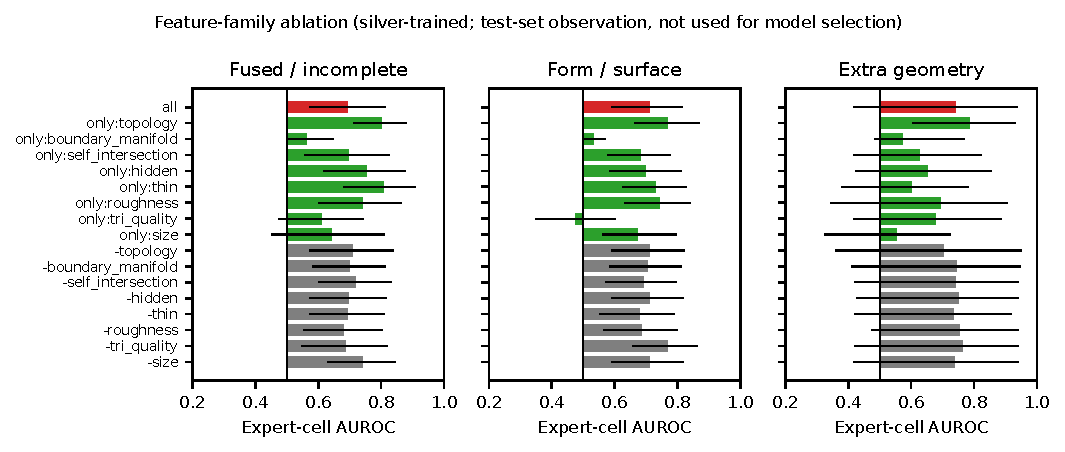
\includegraphics[width=\linewidth]{figures/fig8_ablation_families.pdf}
  \caption{Family-only and leave-one-family-out AUROC on the expert-agreement cells, for models trained on the silver holdout. Topology alone matches or exceeds the full model. That comparison was not used to select the reported predictor.}
  \label{fig:ablate}
\end{figure}
% src: results/ablations/lofo_family_rules.csv

Training on the expert cells does not beat training on the noisy silver labels.
Across 50 repeats of five-fold cross-validation on the agreement cells, expert-trained AUROC is 0.719 against 0.695 for the frozen silver model on fused/incomplete (mean difference \(+0.024\), positive in 68\% of repeats), 0.729 against 0.710 on form/surface (\(+0.019\), 72\% of repeats), and 0.502 against 0.742 on extra geometry (\(-0.240\), positive in 0\% of repeats; six positives).
A model fit on all expert cells and applied to the silver holdout has AUROC 0.599, 0.563 and 0.467, against silver out-of-fold AUROC 0.704, 0.521 and 0.686.
Eighty-eight to 121 expert cells did not outperform 548 crowd labels.
% src: results/RESULTS_milestone2.md; results/ablations/expert_trained_on_silver.csv

Learned fusion does not improve the strong VLMs.
A logistic regression on the frozen probe logit plus the VLM vote, evaluated by 50 repeats of five-fold cross-validation on the expert cells, has mean \(\Delta\)MCC across the 12 VLMs of \(-0.008\) (fused/incomplete), \(+0.107\) (form/surface) and \(0.000\) (extra geometry).
For the four strong VLMs from the paired analysis---Gemini 2.5 Pro, Gemini 3.1 Pro, GPT-5.4 and Claude Opus 4.7---the mean differences are \(-0.060\), \(-0.014\) and \(-0.021\).
An earlier fusion fit on the silver holdout and applied once to the expert cells helps weaker VLMs (mean \(\Delta\)MCC \(+0.08\) on fused/incomplete and \(+0.11\) on extra geometry) and does not help the best one: Gemini 3.1 Pro on fused/incomplete moves from 0.463 to 0.416.
% src: results/RESULTS_milestone2.md; results/ablations/fusion_repeated_cv.csv; results/exploratory_fusion.csv

The training-free AND rule---flag the defect only if the VLM and the frozen probe both do---is the most consistent combination we tried, and it is still a weak result.
\(\Delta\)MCC is positive in 29 of 36 VLM--defect pairs, negative in 4 and zero in 3.
Averaged over those four VLMs, MCC moves from 0.305 to 0.354 on fused/incomplete, from 0.334 to 0.366 on form/surface, and from 0.301 to 0.518 on extra geometry.
After false-discovery correction, 1 of the 36 AND comparisons is significant: Mistral Small 3.1 24B on fused/incomplete (\(\Delta\)MCC \(= 0.168\), [0.063, 0.297]).
The best VLM does not gain on the defect it already wins.
Gemini 3.1 Pro on fused/incomplete moves from 0.463 to 0.450 (\(\Delta\)MCC \(= -0.014\), \([-0.222, 0.182]\)).
The OR rule can move the other way: for that same cell, OR lowers MCC by 0.129 (\([-0.195, -0.072]\); no bootstrap resample out of 10{,}000 had a non-negative difference, so the adjusted value is below \(10^{-3}\)).
Figure~\ref{fig:and} plots the AND differences.
Directionally consistent, underpowered, and not a reason to replace a strong judge.
% src: results/RESULTS_milestone2.md; results/ablations/and_or_rule_bootstrap.csv

\begin{figure}[t]
  \centering
  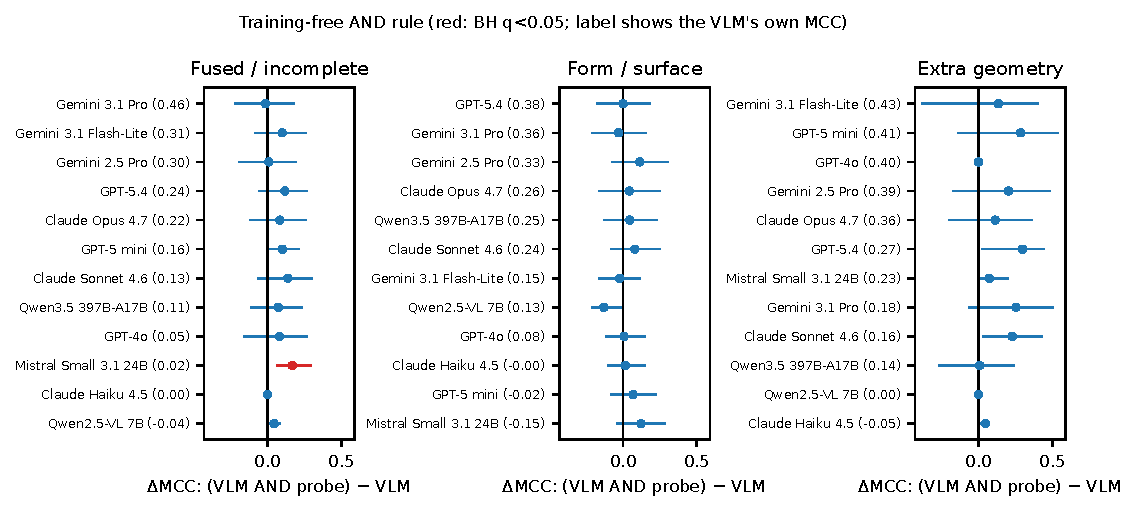
\includegraphics[width=\linewidth]{figures/fig9_and_rule.pdf}
  \caption{Change in MCC when a released VLM vote is conjoined with the frozen probe flag (AND), on the three primary expert-agreement defects. Intervals are bootstrap intervals. One of the 36 comparisons remains significant after Benjamini--Hochberg correction.}
  \label{fig:and}
\end{figure}
% src: results/ablations/and_or_rule_bootstrap.csv; results/RESULTS_milestone2.md

\subsection{Hi3DBench}
\label{sec:hi3d}

Hi3DBench was pre-registered as a secondary, within-generator scale-up.
Its object-level scores are pseudo-labels from the Hi3DEval M$^{2}$AP multi-agent MLLM pipeline, not human ratings \citep{zhang2025hi3deval}.
The primary target, \texttt{geometry\_score}, is Geometry Plausibility.
The secondary target, \texttt{geo\_detail\_score}, is geometric detail.
The four predictors were thin-wall fraction at 0.005, genus proxy, self-intersection fraction and component count, each with a negative predicted sign, on SPAR3D, TRELLIS, TripoSR, InstantMesh, Hunyuan3D and CRM \citep{huang2025spar3d,xiang2025trellis,tochilkin2024triposr,xu2024instantmesh,zhao2025hunyuan3d2,wang2024crm}.
Unique3D was excluded for time and disk budget before scoring \citep{wu2024unique3d}.
We analysed 2{,}797 labelled meshes from 510 image prompts.
Meeting the replication rule here means agreement with that automated judge.
% src: analysis/PREREGISTRATION_M3_hi3dbench.md; results/RESULTS_milestone3.md; results/hi3dbench/hi3dbench_meta.json

All four predictors meet the rule on Geometry Plausibility (Table~\ref{tab:hi3d}, Figure~\ref{fig:hi3d}).
Within generator, thin-wall fraction has Spearman \(\rho = -0.111\) (95\% CI \([-0.157, -0.066]\), adjusted \(p < 0.001\)), genus proxy has \(\rho = -0.063\) (\([-0.106, -0.018]\), adjusted \(p = 0.001\)), self-intersection fraction has \(\rho = -0.042\) (\([-0.084, -0.001]\), adjusted \(p = 0.026\)) and component count has \(\rho = -0.066\) (\([-0.108, -0.025]\), adjusted \(p = 0.001\)).
Every within-generator correlation has absolute value at most 0.111.
The effects are small.
The direction matches the MATE-3D within-generator signs for thin walls, genus and self-intersection, at a smaller magnitude, and it is not a human replication.
% src: results/hi3dbench/hi3dbench_correlations.csv; results/RESULTS_milestone3.md

\begin{table}[t]
  \centering
  \caption{Hi3DBench Geometry Plausibility, an MLLM pseudo-label (\(n = 2{,}797\)). Secondary evidence. \(A\) is the pooled Spearman correlation. \(B\) is the within-generator Spearman correlation (primary), with a prompt-cluster interval. \(q\) is the Benjamini--Hochberg value over the four predictors. \(C\) is mean within-prompt Kendall \(\tau\)-b. \(D\) residualises generator and prompt (2{,}000 bootstrap resamples; the other intervals use 10{,}000). The predicted sign is negative. ``Replicates (B only)'' means \(B\) meets the rule while \(D\) is significantly positive.}
  \label{tab:hi3d}
  \resizebox{\linewidth}{!}{%
  \begin{tabular}{lrrrrrl}
    \toprule
    Predictor & \(A\) & \(B\) [95\% CI] & \(q\) & \(C\) & \(D\) & Verdict \\
    \midrule
    Thin fraction (0.005) & $+0.009$ & $-0.111$ [$-0.157$, $-0.066$] & $<0.001$ & $+0.085$ & $-0.023$ & replicates \\
    Genus proxy & $-0.028$ & $-0.063$ [$-0.106$, $-0.018$] & 0.001 & $+0.033$ & $+0.005$ & replicates \\
    Self-intersection fraction & $+0.022$ & $-0.042$ [$-0.084$, $-0.001$] & 0.026 & $+0.074$ & $+0.044$ & replicates (B only) \\
    Component count & $-0.220$ & $-0.066$ [$-0.108$, $-0.025$] & 0.001 & $-0.175$ & $-0.006$ & replicates \\
    \bottomrule
  \end{tabular}}
\end{table}
% src: results/hi3dbench/hi3dbench_correlations.csv; results/RESULTS_milestone3.md; results/hi3dbench/hi3dbench_meta.json

The within-generator result is not robust to prompt adjustment.
The two-way estimand \(D\) is about zero for thin walls (\(-0.023\), \([-0.067, 0.022]\)), genus (\(+0.005\), \([-0.035, 0.046]\)) and component count (\(-0.006\), \([-0.046, 0.034]\)).
For self-intersection it is positive (\(+0.044\), \([0.005, 0.083]\)), so the interval excludes zero in the direction opposite the prediction.
Between generators the sign flips for thin walls and self-intersection.
Within a prompt, the generator whose mesh has more thin walls, or more self-intersection, tends to receive a higher Geometry Plausibility score (\(C = +0.085\), \([0.051, 0.119]\), and \(C = +0.074\), \([0.034, 0.114]\)).
TRELLIS has by far the highest mean thin-wall fraction (0.185, against at most 0.058 for the other five generators) and the second-highest mean Geometry Plausibility (5.863).
Component count, which the Geometry Plausibility criterion names in connection with floating parts, has the largest pooled and within-prompt associations (\(A = -0.220\), \(C = -0.175\)) and only \(-0.066\) within generator.
% src: results/hi3dbench/hi3dbench_correlations.csv; results/hi3dbench/hi3dbench_per_generator.csv; results/hi3dbench/hi3dbench_meta.json; results/RESULTS_milestone3.md

The per-generator correlations are heterogeneous (Figure~\ref{fig:hi3d}).
They are strongest for CRM, from \(-0.221\) to \(-0.312\) across the four predictors (\(n = 247\)), and for InstantMesh on thin walls (\(-0.214\)) and genus (\(-0.170\)).
They are weaker for Hunyuan3D, SPAR3D and TRELLIS (absolute values at most 0.092).
A single pooled number describes a mixture of these regimes.
% src: results/hi3dbench/hi3dbench_per_generator.csv; results/RESULTS_milestone3.md

\begin{figure}[t]
  \centering
  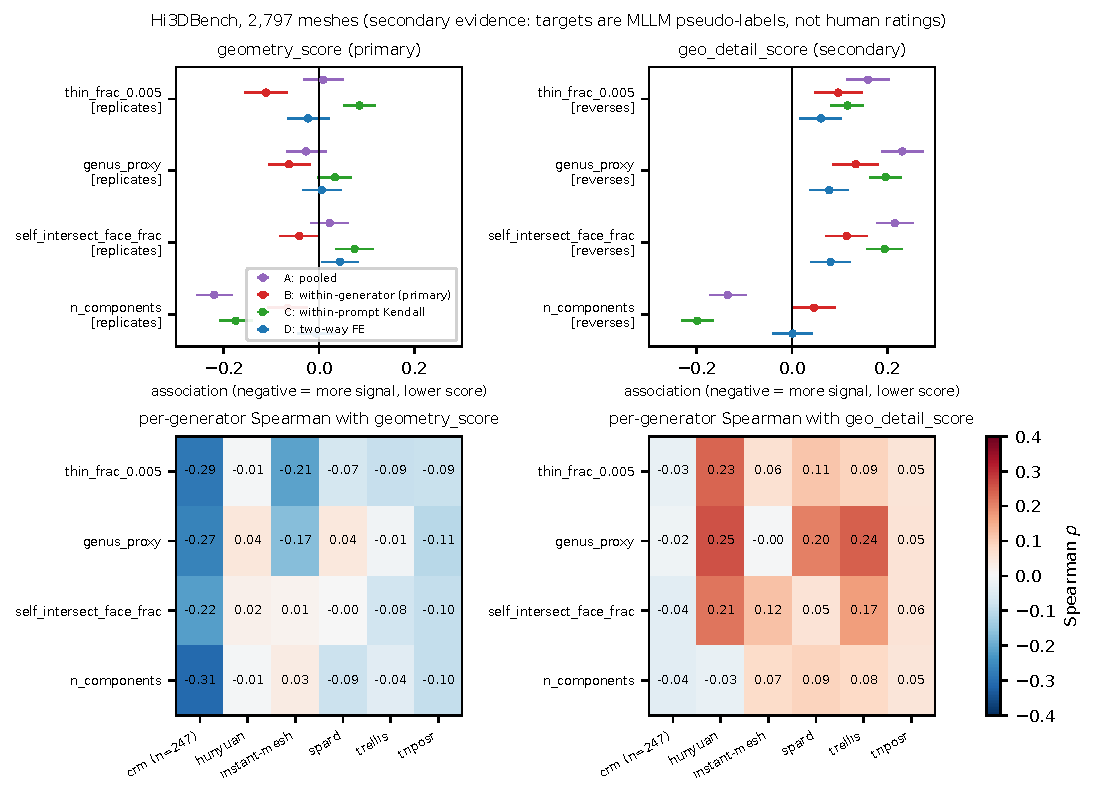
\includegraphics[width=\linewidth]{figures/fig10_hi3dbench.pdf}
  \caption{Hi3DBench, 2{,}797 labelled meshes. Top: estimands \(A\)--\(D\) with prompt-cluster intervals for Geometry Plausibility (primary pseudo-label) and geometric detail (secondary pseudo-label). Bottom: per-generator Spearman correlations. Negative values mean that a larger probe score accompanies a lower pseudo-label. These targets are MLLM outputs, not human ratings.}
  \label{fig:hi3d}
\end{figure}
% src: results/hi3dbench/hi3dbench_correlations.csv; results/hi3dbench/hi3dbench_per_generator.csv; results/RESULTS_milestone3.md

The geometric-detail score reverses all four within-generator signs.
Thin walls, genus, self-intersection and component count have \(\rho = +0.097\) (\([0.047, 0.147]\)), \(+0.134\) (\([0.086, 0.180]\)), \(+0.115\) (\([0.071, 0.158]\)) and \(+0.046\) (\([0.001, 0.092]\)), with adjusted \(p\)-values at most 0.016.
The pooled correlations are \(+0.159\), \(+0.231\), \(+0.216\) and \(-0.135\).
The same ``defect'' signals co-occur with geometric detail as judged by the MLLM pipeline.
That is a complexity confound: a validity gate that penalises thin walls, genus or self-intersection will also penalise meshes this automated judge calls detailed.
% src: results/hi3dbench/hi3dbench_correlations.csv; results/RESULTS_milestone3.md
